\documentclass{article}
\usepackage[final]{neurips_2026}
\makeatletter
\providecommand{\@trackname}{40th Conference on Neural Information Processing Systems (NeurIPS 2026). Competition Track: SimulacraBench.}
\makeatother

\usepackage[utf8]{inputenc}
\usepackage[T1]{fontenc}
\usepackage{hyperref}
\hypersetup{colorlinks=true, linkcolor=black, citecolor=black, urlcolor=blue!50!black}
\usepackage{url}
\usepackage{booktabs}
\usepackage{amsfonts}
\usepackage{amsmath}
\usepackage{amssymb}
\usepackage{nicefrac}
\usepackage{microtype}
\usepackage{xcolor}
\usepackage{graphicx}
\usepackage{enumitem}
\usepackage{array}
\usepackage{tikz}
\usetikzlibrary{positioning,arrows.meta}

\newcommand{\teamid}{Nile}
\newcommand{\todo}[1]{\textcolor{red}{#1}}

\newcommand{\cbox}{$\square$}
\newcommand{\cboxchecked}{$\boxtimes$}

\title{SimulacraBench Technical Report:\\ A Gate-Aware Ensemble for Predicting\\ Survey Responses of Unseen Respondents}

\author{%
  Lkhagvasuren Rentsenbyamba\\
  Bundesdruckerei, Berlin, Germany\\
  \texttt{lkhagvasuren.rentsenbyamba@bdr.de}
  \And
  Nina Ihde\\
  Bundesdruckerei, Berlin, Germany\\
  \texttt{nina.ihde@bdr.de}
}

\begin{document}

\maketitle

\begin{center}
\begin{tabular}{l}
\toprule
\textbf{Team ID:} \teamid \\
\bottomrule
\end{tabular}
\end{center}

\begin{abstract}
We predict the answers of held-out survey respondents from their \texttt{GIVEN} block. Each gated
item is decomposed into the probability of being asked and the answer distribution given that it
was asked; the former comes from the parent item's prediction and gate tables estimated from the
data, because the delivered files do not always follow the questionnaire routing. About 30
conditional models from six families (hierarchical backoff and profile matching, multi-task softmax
networks, latent class and latent factor models, gradient boosting and random forests, an ordinal
logit, and TabPFN~v2) are fitted inside the submission on the visible respondents and combined by a
per-item linear pool with EM-fitted weights and temperature calibration. Structure-aware corrections
for gate parents, multi-select families and ordinal scales are kept only where they improve the
out-of-fold score. A scheduler times every component against the compute budget and falls back to
averaged fold models when a final refit would overrun. Test-phase Grand Prize score:
0.48 (UNICEF 0.34, World Bank 0.23, UNHCR 0.86).
\end{abstract}

%% ---------------------------------------------------------------------------
\section{Method summary}
\label{sec:method}

\subsection{Method type}
Mark every category that applies; the categories are not mutually exclusive. A one-line description of each marked component follows in Section~\ref{sec:pipeline}.

\begin{table}[h]
  \centering
  \small
  \resizebox{\textwidth}{!}{%
  \begin{tabular}{@{}clcl@{}}
    \toprule
    \cbox & LLM-simulated respondents (prompting, personas) & \cbox & Fine-tuned language model \\
    \cboxchecked & Tabular / conditional generative model (e.g.\ VAE, diffusion, GAN, CTGAN) & \cboxchecked & Supervised prediction (GBDT, neural net, linear/GLM) \\
    \cboxchecked & Bayesian / hierarchical / multilevel model & \cboxchecked & Small-area estimation or post-stratification (e.g.\ MRP) \\
    \cbox & Reweighting, raking, or calibration of the released sample & \cboxchecked & Imputation / matching / nearest-neighbour \\
    \cbox & Retrieval over released or external microdata & \cbox & Agent-based or mechanistic simulation \\
    \cboxchecked & Ensemble or stacking of multiple components & \cboxchecked & Other: pretrained tabular model (TabPFN~v2) \\
    \bottomrule
  \end{tabular}}
\end{table}

\subsection{Pipeline}
\label{sec:pipeline}
The submission is a single \texttt{predict(frame, schema)} function. All fitting happens inside it,
once per instrument, on the visible (complete) respondents; nothing is trained offline except the
pretrained TabPFN~v2 checkpoint~\citep{hollmann2025tabpfn}. Figure~\ref{fig:pipeline} shows the steps.

\begin{figure}[h]
  \centering
  \small
  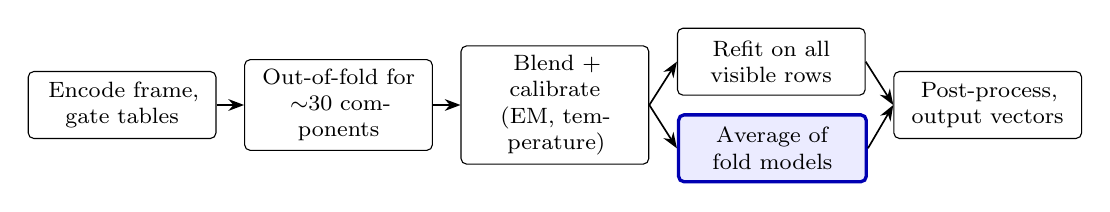
\begin{tikzpicture}[
      box/.style={draw, rounded corners=2pt, align=center, minimum height=0.85cm, text width=2.15cm, font=\footnotesize},
      acc/.style={box, draw=blue!70!black, fill=blue!8, very thick},
      arr/.style={-{Stealth[length=2mm]}, semithick}, node distance=0.35cm]
    \node[box] (enc) {Encode frame,\\ gate tables};
    \node[box, right=of enc] (oof) {Out-of-fold for\\ $\sim$30 components};
    \node[box, right=of oof] (bl) {Blend + calibrate\\ (EM, temperature)};
    \node[box, right=of bl, yshift=0.55cm] (rf) {Refit on all\\ visible rows};
    \node[acc, right=of bl, yshift=-0.55cm] (fa) {Average of\\ fold models};
    \node[box, right=of rf, yshift=-0.55cm] (pp) {Post-process,\\ output vectors};
    \draw[arr] (enc) -- (oof);
    \draw[arr] (oof) -- (bl);
    \draw[arr] (bl.east) -- (rf.west);
    \draw[arr] (bl.east) -- (fa.west);
    \draw[arr] (rf.east) -- (pp.west);
    \draw[arr] (fa.east) -- (pp.west);
  \end{tikzpicture}
  \caption{Pipeline per instrument. A component is kept only if its timed first fold predicts that all folds and the refit fit the budget; a refit that would overrun is replaced by the average of the fold models (lower path).}
  \label{fig:pipeline}
\end{figure}

\subsection{Inputs and feature construction}
The method uses only the \texttt{GIVEN} columns of each respondent and the answers of the visible
respondents. \texttt{respondent\_id}, row order, question wording and \texttt{EXCLUDE} items are not
used. Every option is coded by normalised string (so \texttt{3}, \texttt{3.0} and \texttt{"3"}
agree); \texttt{GIVEN} columns become a one-hot matrix for the linear, neural and latent models and
stay as codes for trees and count models. A profile-matching model never lets the survey-round
column differ, so no household is matched with its own record from another round.

\subsection{Model or simulator}
For a gated item $j$ with \texttt{GIVEN} block $x$,
\begin{equation*}
P(y_j = v \mid x) = P(\text{asked}_j \mid x)\, P(v \mid \text{asked}_j, x), \quad
P(y_j = \texttt{NA\_GATED} \mid x) = 1 - P(\text{asked}_j \mid x).
\end{equation*}
$P(\text{asked}_j \mid x) = \sum_v P(\text{parent} = v \mid x)\, t_j(v, c(x))$, where $t_j$ is an
empirical table over the parent value and up to two context columns $c(x)$ (typically the survey
round), shrunk toward the schema rule. Context columns are added greedily by bias-corrected
conditional mutual information. Items are composed in topological order of the gates. Several
components also exist in a \emph{direct} variant that treats \texttt{NA\_GATED} as an ordinary
answer. The conditional models are: smoothed marginals; hierarchical Dirichlet backoff over up to
three \texttt{GIVEN} columns; profile matching on identical or near-identical profiles; multi-task
softmax regression and MLPs; latent class regression~\citep{dayton1988concomitant}; a continuous
latent factor model (multidimensional nominal-response IRT~\citep{bock1972nominal} fitted as a
VAE~\citep{kingma2014vae}); per-item gradient boosting and a multi-output random
forest~\citep{breiman2001rf,pedregosa2011sklearn}; a proportional-odds
logit~\citep{mccullagh1980ordinal}; and TabPFN~v2 per item. Questions are treated as conditionally
independent given $x$, which is exact for the per-cell log score. Appendix~\ref{app:config} lists
every component with its settings.

\subsection{Fitting, training, or prompting}
Everything is fitted at run time on the visible rows (TRAIN in the development phase, TRAIN and DEV
in the test phase); no external data. Out-of-fold predictions come from 3 folds (development) or 5
folds (test). Linear models and MLPs use full-batch L-BFGS with output biases initialised at the log
marginals; boosting uses early stopping on 15\% of the rows; backoff and profile-matching strengths
are chosen per item by exact leave-one-out log score. A scheduler times each component's first fold
and drops it if all folds plus the refit would exceed 85\% of the instrument's budget.

\subsection{Prediction and aggregation}
The components' out-of-fold distributions are combined by a linear pool whose weights are fitted per
item by EM~\citep{dempster1977em} on the floored log likelihood (floor 0.001, as in the grader),
shrunk toward per-instrument weights (Dirichlet prior, strength 30). Final predictions come from
components refitted on all visible rows, or from the average of their fold models when the refit
would not finish in time. There are no survey weights to apply.

\subsection{Post-processing and calibration (if applicable)}
Fitted on the out-of-fold blend and applied only where they improve its log
score~\citep{gneiting2007scoring}: one temperature per instrument and optionally per
item~\citep{guo2017calibration}; temperatures of gate parents chosen on the parent's and its
children's log scores; for multi-select families, a common logit shift that ties each respondent's
expected number of ticks to the observed relation with the predicted count; and smoothing of
probability mass between neighbouring bands of numeric scales.

%% ---------------------------------------------------------------------------
\section{Models, data, and compute}
\label{sec:resources}

\paragraph{Pretrained models and off-the-shelf components.}

\begin{table}[h]
  \centering
  \small
  \caption{Pretrained models and off-the-shelf components.}
  \label{tab:models}
  \begin{tabular}{>{\raggedright\arraybackslash}p{3.0cm}>{\raggedright\arraybackslash}p{5.4cm}>{\raggedright\arraybackslash}p{4.0cm}}
    \toprule
    Component & Version / checkpoint & Role in pipeline  \\
    \midrule
    TabPFN v2 classifier (Prior Labs License) & \texttt{Prior-Labs/TabPFN-v2-clf} at commit \texttt{f851f2a}, file \texttt{tabpfn-v2-classifier.ckpt}; package \texttt{tabpfn==9.1.0} & per-item in-context classifier in the ensemble \\
    scikit-learn & version of the hosted image & gradient boosting, random forest \\
    \bottomrule
  \end{tabular}
\end{table}

\paragraph{Data.} Only the official SimulacraBench frames passed to \texttt{predict}; the organisers'
synthetic sandboxes were used for local development and timing. No external data.

\begin{table}[h]
  \centering
  \small
  \caption{External datasets used.}
  \label{tab:external}
  \begin{tabular}{llll}
    \toprule
    Dataset & Source / URL & Size & Use in pipeline \\
    \midrule
    None & -- & -- & -- \\
    \bottomrule
  \end{tabular}
\end{table}

\paragraph{Compute.} One H100 and 8 CPU cores of the hosted container. The total budget (our own
limit: 780\,s development, 3300\,s test) is split across instruments in proportion to their measured
cost. In a local test-phase simulation the full run took about 2{,}700--2{,}850\,s with a peak memory
of 5.2\,GB.

%% ---------------------------------------------------------------------------
\section{Results}
\label{sec:results}

\subsection{Test-phase leaderboard results}

\begin{table}[h]
  \centering
  \small
  \caption{Official SimulacraBench results for team \teamid{} (skill relative to the crowd marginal).}
  \label{tab:results}
  \begin{tabular}{lrrrr}
    \toprule
    Split & Grand Prize & UNICEF & World Bank & UNHCR \\
    \midrule
    Development & 0.48 & 0.35 & 0.25 & 0.85 \\
    Test        & 0.48 & 0.34 & 0.23 & 0.86 \\
    Organizer baseline (test) & 0.000 & 0.000 & 0.000 & 0.000 \\
    \bottomrule
  \end{tabular}
\end{table}

\subsection{Breakdown by population, survey, or question type}
UNHCR, the instrument with the most structure (213 items, 156 of them gated, 139 options of
multi-select questions), is where modelling choices mattered most. On the development leaderboard
(original uniform-reference skill), modelling the skip logic with context-dependent gate tables
raised UNHCR from 0.76 to 0.90, and gradient boosting on every item to 0.92; UNICEF (0.52) and World
Bank (0.49) did not move in any version. UNHCR remains our weakest instrument relative to the
leaders (0.85 vs.\ 0.87 on the marginal-reference development scale).

%% ---------------------------------------------------------------------------
\section{Reproducibility}
\label{sec:repro}

\begin{itemize}[leftmargin=*]
  \item Code repository: \url{https://github.com/Lxagvaa/simulacrabench-nile} (licence: MIT)
  \item Commit hash used for the test-phase submission:\\ \texttt{f206a15a3e47bf5457abb6968153ecdcdc2aee17}
  \item Command to reproduce the test-phase submission file: \texttt{make setup \&\& make zip}
        (builds and validates \texttt{dist/submission.zip}); \texttt{make eval-final} runs it under
        test-phase conditions on the organisers' sandboxes.
  \item Environment: Python with \texttt{uv}; dependencies in \texttt{pyproject.toml} and
        \texttt{uv.lock}; the hosted image provides torch and scikit-learn; \texttt{requirements.txt}
        pins \texttt{tabpfn==9.1.0}.
  \item Pretrained weights: TabPFN~v2 checkpoint, downloaded by \texttt{scripts/fetch\_weights.sh}
        from Hugging Face at the pinned commit and checked by SHA-256; publicly available.
\end{itemize}
Seeds are fixed. Because the scheduler drops components by measured time, the set of components
that run, and hence the predictions, can differ slightly on other hardware.

%% ---------------------------------------------------------------------------
\section{Limitations}
\label{sec:limitations}

The method predicts each cell from the \texttt{GIVEN} block alone, so it cannot do better than the
information those few columns carry; on UNICEF and World Bank all strong teams converged on almost
the same score. Its gains were validated mostly on out-of-fold scores and synthetic data, where they
translated to real data at roughly a third of their size, so small differences between its
components should not be over-interpreted.

%% ---------------------------------------------------------------------------
\bibliographystyle{plainnat}
\bibliography{refs}

%% ---------------------------------------------------------------------------
\clearpage
\appendix

\section{Full configuration}
\label{app:config}

\paragraph{Components} in priority order (the scheduler keeps them while they fit the budget).
``Direct'' variants predict \texttt{NA\_GATED} as an ordinary answer instead of using the gate
decomposition.

\begin{table}[h]
  \centering
  \small
  \begin{tabular}{p{3.6cm}p{9.2cm}}
    \toprule
    Component & Settings \\
    \midrule
    Marginal & answer shares among respondents asked, +0.5 pseudo-count \\
    Backoff, depth 1/2/3 & Dirichlet shrinkage over \texttt{GIVEN} strata; columns by bias-corrected conditional MI; $\alpha \in \{0.5,\dots,64\}$ per item by leave-one-out \\
    Linear (multi-task softmax) & L2 $10^{-2}$ and $10^{-3}$; one variant with one-hot cells for all pairs of the 5 most informative columns (cells $\geq 20$ rows), one with 7 columns and L2 $3\cdot10^{-3}$ \\
    MLP & one tanh layer of 64 or 128 units, L2 $3\cdot10^{-3}$, three seeds; L-BFGS, 250 iterations \\
    Latent class regression & $K = 8, 16$; EM up to 80 iterations; class model multinomial logit, L2 $10^{-2}$; item tables smoothed toward marginals \\
    Factor VAE & $d = 3, 5$; encoder one tanh layer of 128 units on \texttt{GIVEN} + answers; prior $N(Gx, I)$; Adam, lr $3\cdot10^{-2}$, 400 epochs; 64 Monte Carlo samples at prediction \\
    Gradient boosting & per item, HistGradientBoosting, native categoricals, early stopping (15\%, patience 10); default: lr 0.15, 150 iterations, 15 leaves, min leaf 20, L2 1; deep: 31 leaves, min leaf 10; big: 63 leaves, min leaf 5, lr 0.1, 300 iterations, L2 0.5; default and deep also direct \\
    Random forest & multi-output, 100 trees, min leaf 5, 50\% features and rows per tree \\
    Profile matching & identical profile, then profiles differing in one non-round column, shrunk toward depth-3 backoff; strengths by leave-one-out; also direct \\
    Ordinal logit & proportional odds over substantive options, L2 $10^{-2}$; non-substantive options keep their marginal share \\
    TabPFN v2 & one ensemble member on all items with $\leq 10$ classes; four members on the 40 top-ranked items (development) or all items (test); $\leq 10{,}000$ context rows \\
    \bottomrule
  \end{tabular}
\end{table}

\paragraph{Gate model.} Prior: schema rule with confidence 0.995 and strength 2; context levels
shrunk toward the coarser level with strength 10; at most two context columns. Per-item heavy models
(boosting, TabPFN) cover gate parents first, ranked by the number of dependent items.

\paragraph{Blend and calibration.} EM from 2{,}000 iterations (global, started at 80\% weight on the
best single component) and 300 iterations per item; temperature in $[0.6, 1.5]$, per item only if
the out-of-fold gain exceeds 2 nats. Post-processing steps require out-of-fold gains of 5 nats (gate
parents, multi-select families) or 2 nats (ordinal smoothing).

\paragraph{Time and memory.} Each fit checks a wall-clock deadline; L-BFGS evaluations are capped
at $3\times$ the iteration limit; boosting fits run single-threaded, eight items in parallel; one
TabPFN network is shared across items; if a crash reaches the entry point, crowd marginals are
returned for that instrument.

\section{(Optional) Additional results}

\paragraph{What did not help.} Learned gate parents (no gain: the direct variants already predict
\texttt{NA\_GATED} from \texttt{GIVEN}); adapting to a visible/held-out shift (never triggered, as
roles were assigned after shuffling); a log-linear instead of linear pool ($-0.0014$ to $+0.0009$
skill); stacking a second stage on all items' predictions (out-of-fold gains did not transfer).

\end{document}
